\documentclass[man,noapacite]{apa2} 

\usepackage{url}
\usepackage{apacite2}
\usepackage{amssymb}
\usepackage{graphicx}

\title{Wordbank: An Open Repository for Developmental Vocabulary Data} 

\author{Michael C. Frank, Mika Braginsky, Daniel Yurovsky, \& Virginia Marchman} 

\affiliation{Department of Psychology, Stanford University}

\abstract{Understanding the processes by which vocabulary grows provides a window into linguistic and cognitive development. The MacArthur-Bates Communicative Development Inventories (CDIs) are a widely-used family of parent-report instruments for easy and inexpensive data-gathering about early language acquisition. CDI data have been used to explore a wide variety of theoretically-important topics, but with few exceptions, researchers have had to rely on data collected in their own lab: there is no resource that offers researchers the opportunity to share and access raw CDI data. We describe Wordbank, a structured database of item-by-child data of vocabulary measures from CDI forms combined with a browsable web interface. Wordbank archives CDI data across languages and labs, providing a resource for researchers interested in early language as well as a platform for novel analyses.}

\shorttitle{Wordbank: A Repository For Vocabulary Data} 
\rightheader{WORDBANK: A REPOSITORY FOR VOCAB DATA}

\acknowledgements{This work supported by a John Merck Scholars award to MCF and NSF \#XYZ. Please address all correspondence to Michael C. Frank, Department of Psychology, Jordan Hall (Bldg. 420), 450 Serra Mall, Stanford, CA 94305. Phone: (650) 724-4003. E-mail: \texttt{mcfrank@stanford.edu}}

\begin{document}

\maketitle


\section{Introduction}


Learning language is one of the most impressive and intriguing human accomplishments: A child's first words are eagerly awaited by parents, dutifully recorded in baby books, and celebrated with family and friends. Early achievements in vocabulary are correlated with subsequent progress in grammar \cite{bates1999}, and understanding the processes by which vocabulary grows provides a window into mechanisms of linguistic and cognitive development more generally \cite{bloom2002}. In addition, since vocabulary growth lays the groundwork for future academic achievement \cite{hart1995,marchman2008}, a better scientific understanding of vocabulary holds the promise of societal benefits.

The MacArthur-Bates Communicative Development Inventories \cite<CDIs;>{fenson1994,fenson2007} are a widely-used family of parent-report instruments for easy and inexpensive data-gathering about early language acquisition. CDI data have been used to explore many theoretically-rich topics, including variation in early word production \cite{fenson1994}, vocabulary composition \cite{bates1994}, and the growth of lexical networks \cite{hills2009}. With few exceptions, however, researchers have had to rely on data collected in their own lab. While CDI norms are available \cite{fenson2007,jorgensen2010}, no resource offers researchers the opportunity to share and access raw, cross-linguistic data at the scale necessary to address questions about demographic variation, vocabulary composition, relations with grammatical development, and other important issues.

To remedy this issue, we introduce Wordbank (\url{http://wordbank.stanford.edu}), a structured database of developmental vocabulary data. Wordbank archives CDI data across languages and labs, providing an large-scale database of information about children's vocabulary knowledge. The site hosts an interactive and expandable set of in-depth analyses that can be explored by interested researchers, students, and members of the public. Wordbank lowers the cost of new, exploratory analyses by facilitating the productive reuse of data that have already been collected by researchers.

In the current paper, we begin by describing the motivations for Wordbank. The bulk of the paper then describes the wordbank site, including its database architecture, its web-based front-end, and methods for extending the site. We next describe \texttt{wordbankR}, a package for the \texttt{R} statistical programming language that allows research users to access the database directly. We end by discussing possible directions for the expansion of Wordbank.

\section{Motivation and Background} 

For researchers, the nature and course of early word learning is a window into the child's growing understanding of the world around her and provides critical information regarding the mechanisms which guide the construction of a rich and structured lexicon and the subsequent development of grammar. Infants typically begin to associate sound sequences with meanings toward the end of their first year of life, responding appropriately to familiar phrases, such as ``It's time for bath!'' (e.g., by plopping down and attempting to remove their shoes); the production of recognizable words begins somewhat later. Early words cross-cut a variety of linguistic categories, but generally consist of names for caregivers (e.g., mama), common objects (e.g., bottle, shoe), social expressions (e.g., bye-bye), and actions or routines (e.g., peekaboo, throw) \cite{nelson1973,tardif2008}. 

New words tend to enter children's expressive vocabularies over the next several months slowly but steadily: children reach reach an average of 300 words by 24 months and more than 60,000 by the time they graduate from high school \cite{fenson2007}. At the same time, there are significant individual differences in language acquisition, as documented by early diary and observational studies, techniques with a long and respected history in the field of child language. For example, although some 18-month-olds already produce 50--75 words, others produce no words at all, and will not do so until they are 22 months or older \cite<e.g.,>{brown1973}. 

\subsection{Measuring early vocabulary}

Traditional studies of language development typically apply a combination of observational assessment and structured tests, frequently relying on short samples of interactions and small samples of children. However, discerning both the universal features and natural variation of language development has been greatly facilitated by the development of parent report instruments like the MacArthur-Bates CDI \cite{fenson1994,fenson2007} and the Language Development Survey \cite{rescorla1989}. The CDIs were developed across a period of more than 40 years. Originally designed for use in a research study \cite{bates1976}, the instruments evolved from a structured interview to the current paper-and-pencil format. 

While many other more sophisticated assessment tools exist for slightly older children (e.g. the PPVT; \citeNP{dunn2007}), to our knowledge, no measure allows cost-effective global language assessment for children in the critical age ranges between the emergence of language and the period when children become more able to perform long-form tasks at around 30 months. Naturalistic observations are the leading candidate, but such observations are extremely costly and difficult to transcribe and annotate. In addition, estimates of vocabulary from naturalistic observation are highly correlated with the CDI within studies \cite<e.g.>{bornstein1998}, but affected substantially by length of the session, context, and interlocutor across studies.

The CDI takes advantage of the fact that parents are expert observers of their child. CDI instruments ask about use of communicative gestures, grammar, and symbolic play, as well as vocabulary, which is measured using checklists consisting of representative samples of words. Parents choose the words their child currently ``understands'' (comprehension) or ``says'' (production).  The checklists contain words from many different semantic (e.g., animals names, household items) and grammatical (e.g., action words, connectives) categories, resulting in broader samples of lexical knowledge than are available from other methods. The long forms of the instruments come in two versions: Words \& Gestures (8--18 months) and Words \& Sentences (16--30 months). Originally designed for English, parallel instruments have now been adapted for more than 60 languages.

% Parent reports have several advantages over other assessments of children's language skill: 

% \begin{itemize}
% \item Because the parent has the opportunity to observe their child in a wide range of situations, parents can provide data that are more representative of the child's actual language knowledge than can be observed in a laboratory sample.
% \item Parent reports may be less influenced by aspects of a child's personality or mood that can interfere with lab-based testing.
% \item Easy-to-administer, paper-and-pencil checklists like the CDI make it feasible to assess communicative behaviors in much larger samples than those typically used in experimental or observational child language research.
% \item The parent report methodology is a fruitful and practical way to conduct studies of child language from a cross-linguistic perspective, as is evident by dozens of currently-available adaptations to languages other than English.
% \end{itemize}


Over the last several years, the technique of parent report has continued to gain popularity. In addition to standard research projects, which frequently include the CDI as an auxiliary outcome or control measure, the CDI instruments have been adopted in a variety of large-scale studies both in the US (e.g., the NICHD Study of Early Child Care) and in other countries. This broad and deep use of CDI forms creates a moment of opportunity: Although the CDI has many users, to perform new analyses of a topic of interest, researchers still typically collect their own sample, and the size and composition of these samples is limited.

\section{Wordbank}

To remedy this situation, we present the Wordbank website. The current main page of the site is shown in Figure \ref{fig:screenshot}. We begin by describing technical details of the site's database architecture. We then describe the two primary analyses that form the heart of the site's interactive functionality. We end by discussing the extensibility of the wordbank framework, highlighting opportunities for contributing data and for building new analyses. 

\begin{figure}[h!]
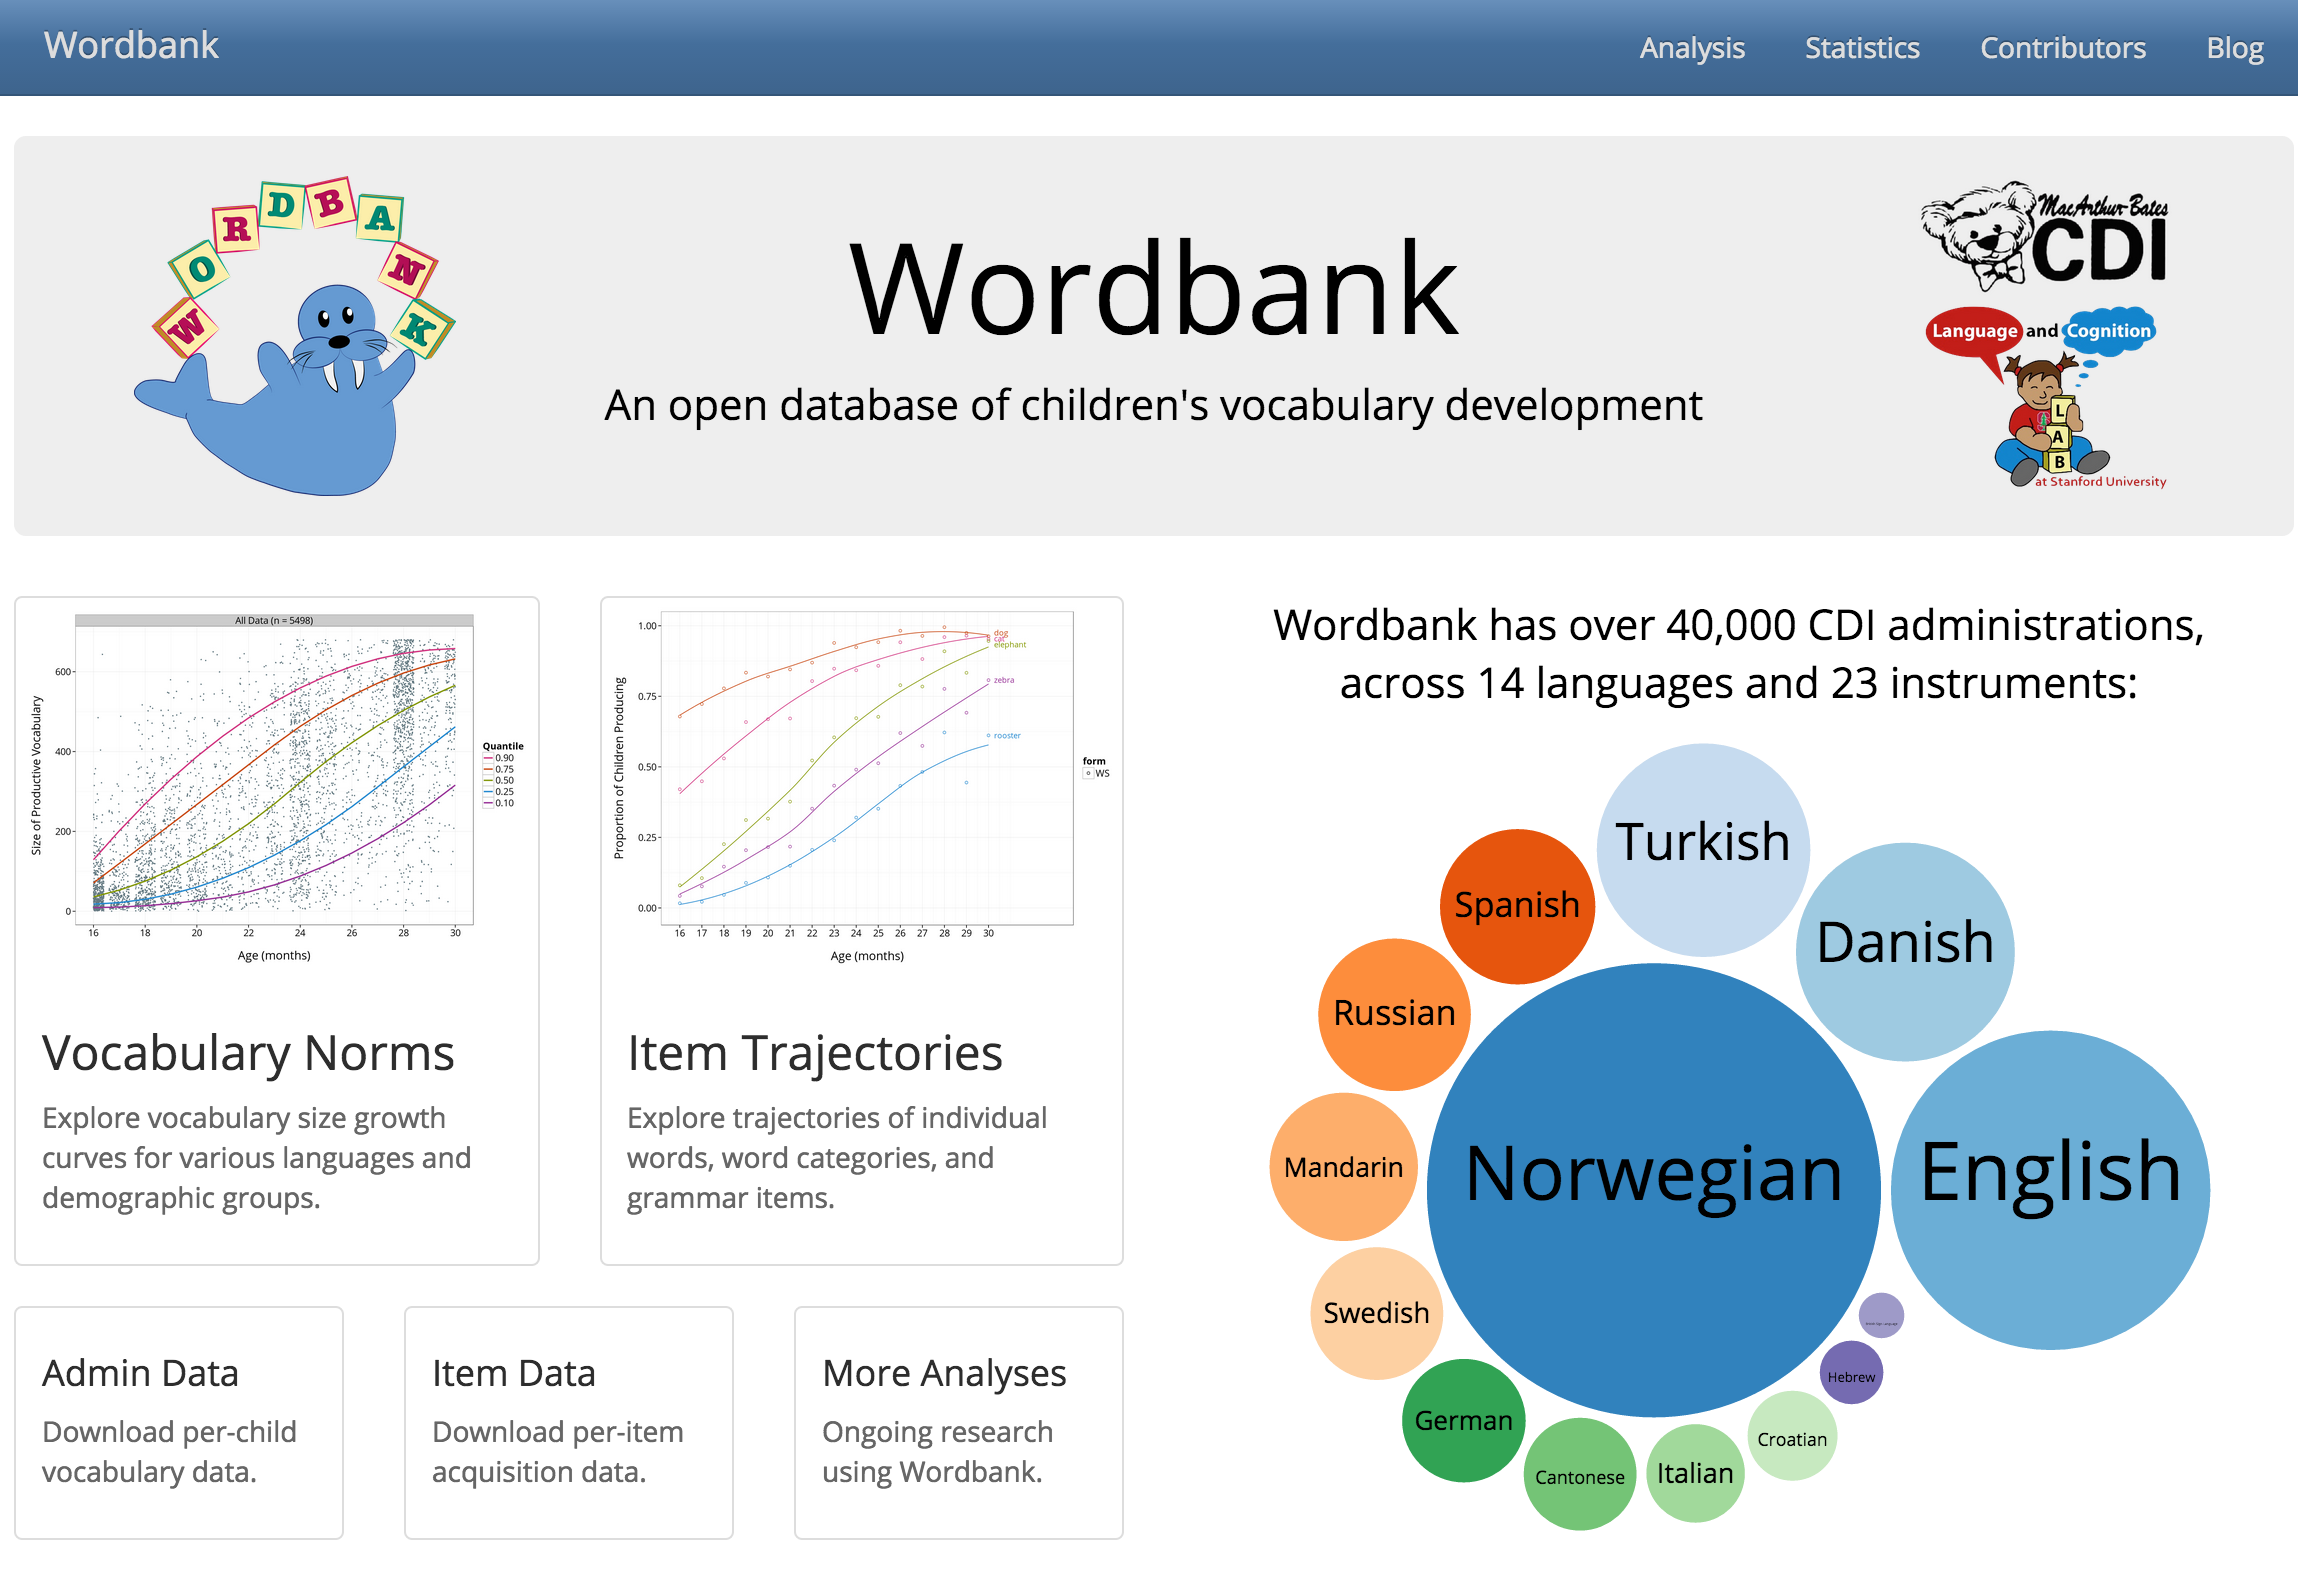
\includegraphics[width=6.4in]{figures/screenshot.png}
\caption{\label{fig:screenshot} Screenshot of the current Wordbank main page. Visitors can navigate from this page to the interactive reports, as well as to a statistics page that shows the database composition, a contributors page that shows citation information, and a blog that highlights recent updates.}
\end{figure}

\subsection{Database Architecture}

\begin{figure}[t]
\centering
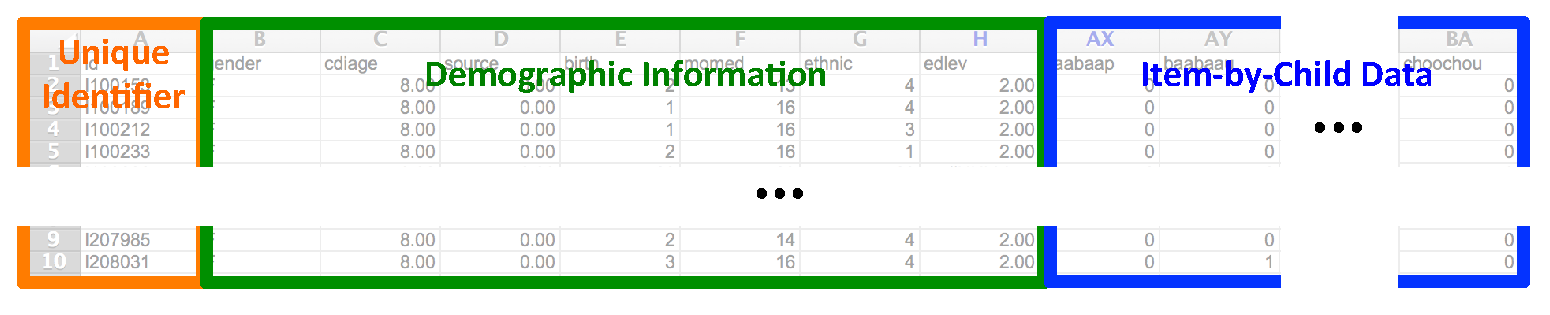
\includegraphics[width=5in]{figures/itembychild.pdf}
\caption{\label{fig:data} Example item-by-child data from the CDI norming sample (Fenson et al., 2007). Each row has a unique child identifier, demographics, and word-by-word checklist data. }
\end{figure}

Why use a database to store vocabulary data? Consider the standard format of item-by-child CDI data. Figure \ref{fig:data} shows a small slice of the original CDI norming data \cite{fenson1994,fenson2007}. Each row is a child, each column gives a variable---either a demographic variable or the result of a particular word being administered to a particular child. Although this format is useful for homogeneous administrations of a single instrument, it cannot accommodate multiple instruments, multiple languages, or datasets with different sources or kinds of demographic information. Consolidating data across different instruments is very difficult in this format, and tracking data on children with multiple longitudinal administrations of a single instrument must also be done in an ad-hoc manner. The move to a database format allows far more flexible and programmatic handling for heterogeneous data structures from different sources. 

A relational database such as Wordbank is at its heart a series of tables linked by unique identifiers. Wordbank's organization is shown in Fig. \ref{fig:entities}. The primary table is the \emph{administrations} table, which catalogs each administration of a given CDI instrument to a particular child at a particular age. The \emph{child} table describes the demographics of the child, including---but not limited to---sex, birth order, mother and father's education, place of testing (country or US state), birth weight, etc. The \emph{source} table gives the contributor and (where relevant) published citation for the particular CDI administration. This is the tag by which contributors can re-export their own particular data.


\begin{figure}[t]
\centering
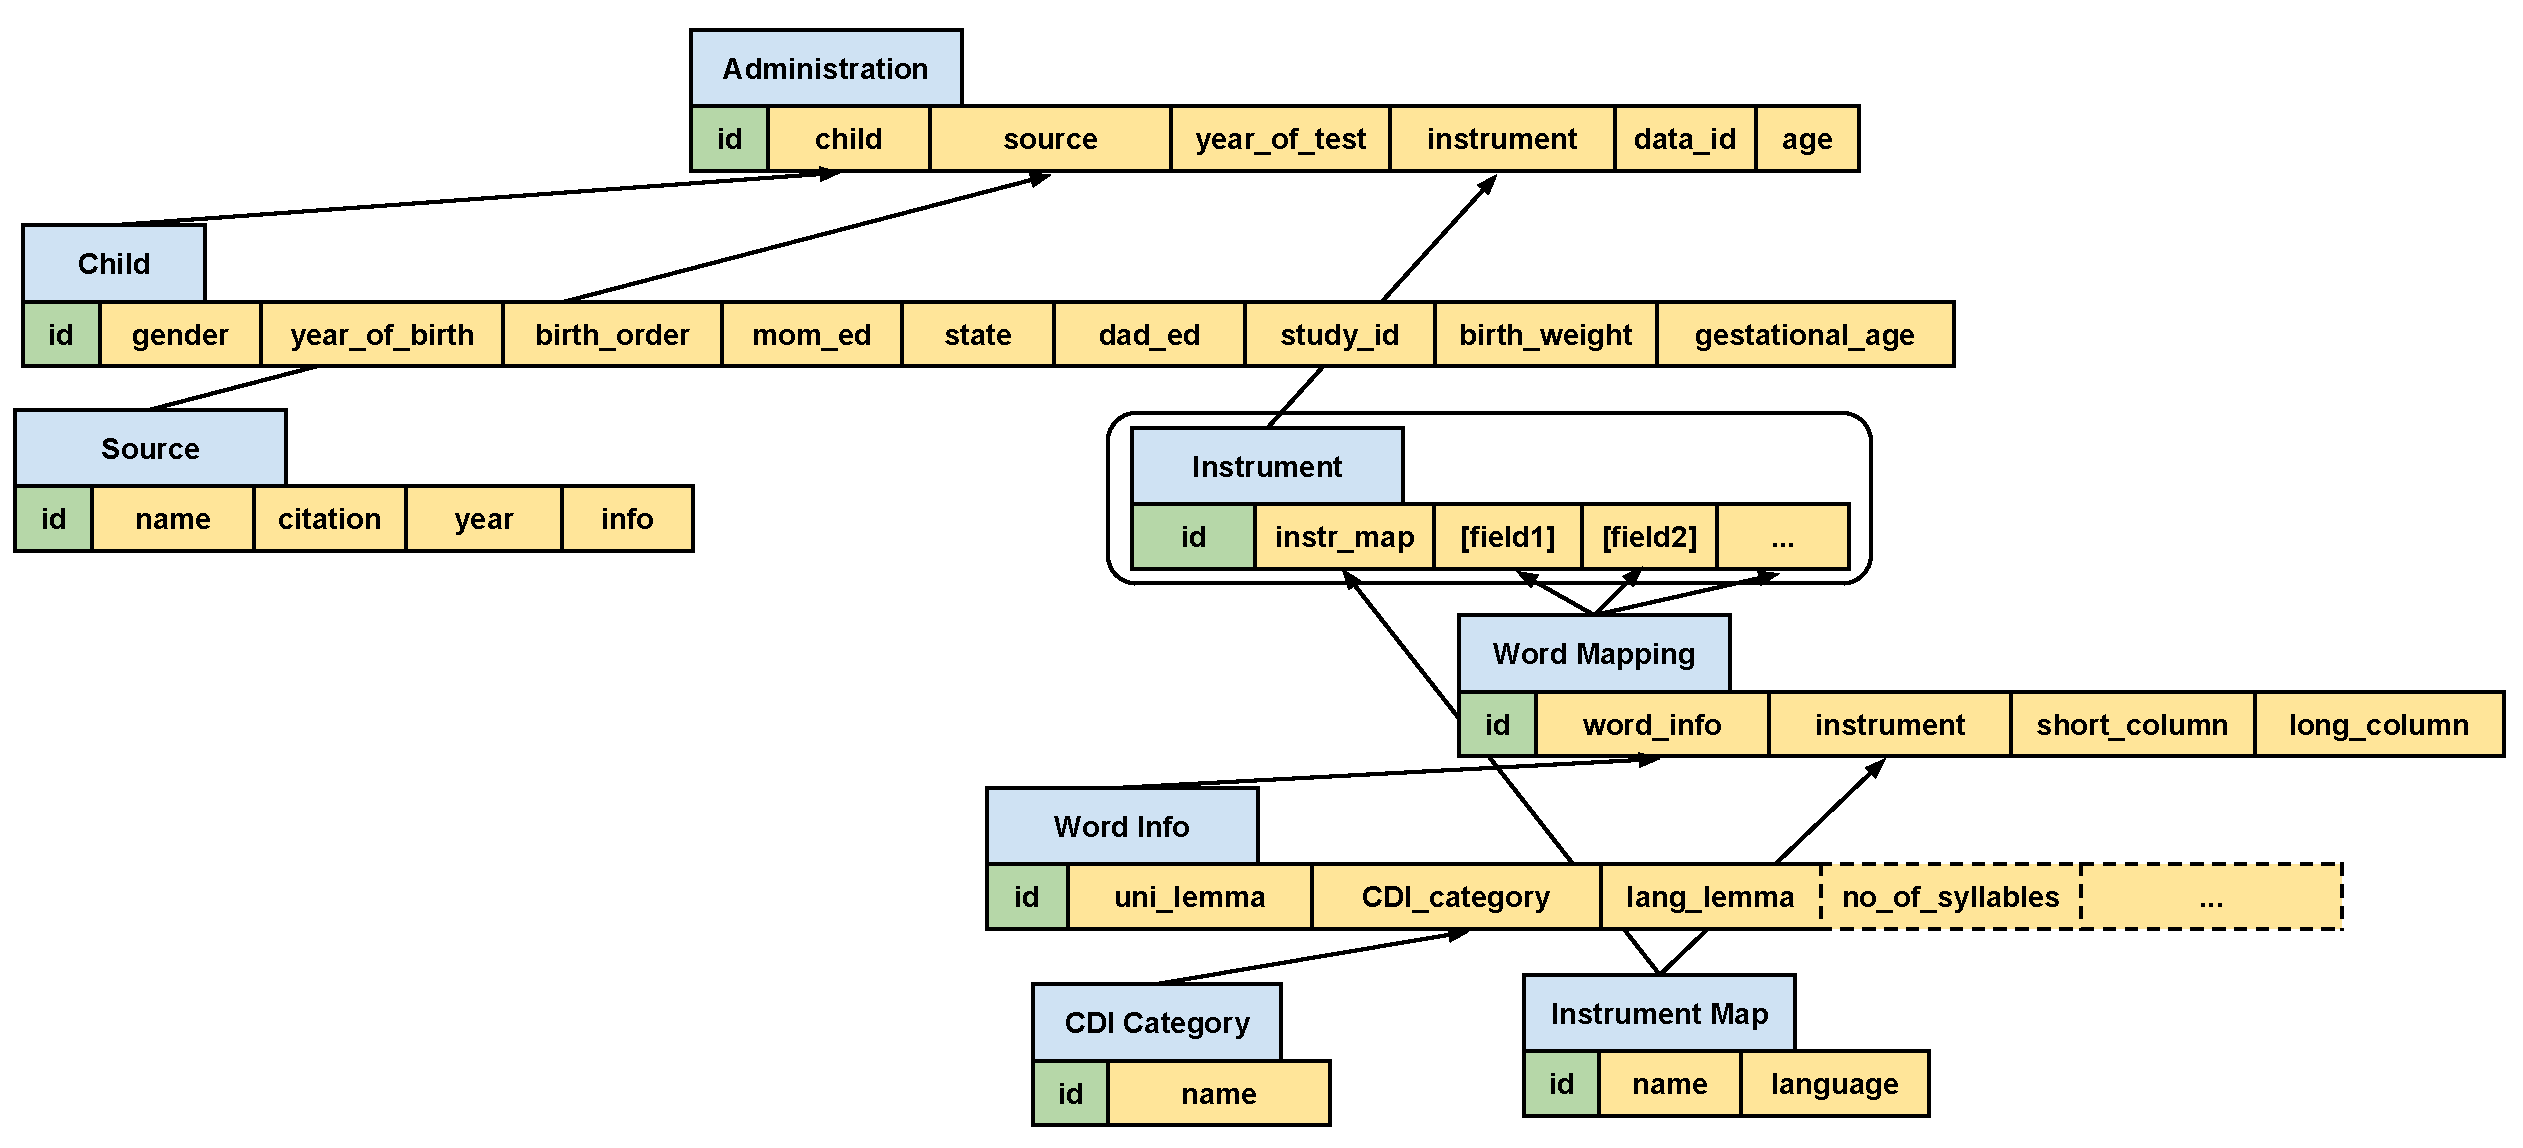
\includegraphics[width=4.5in]{figures/entities.pdf}
\caption{\label{fig:entities} Entity-relation diagram for the Wordbank database. The fundamental table administrations, in which an instrument (a CDI form) is used to measure vocabulary for a child by a particular source (researcher or lab). Instruments are se!s of words, each be linked to descriptive information, including categories and norms.}
\end{figure}

CDI instruments in Wordbank are organized through linked tables: the \emph{instrument} table gives the words in each instrument, while the \emph{word info} table contains information about each word, including number of syllables, number of phonemes, frequency in a corpus, psycholinguistic norms, or any other variables relevant to analyses of vocabulary growth. The \emph{CDI category} table is used to provide categorizations of words into relevant groupings for further category-based analysis.

\subsection{Interactive Analyses}

The primary method for users to interact with the Wordbank is through interactive reports that are hosted on the website. These reports allow exploration of 

\subsubsection{Vocabulary Norms}

\begin{figure}[h!]
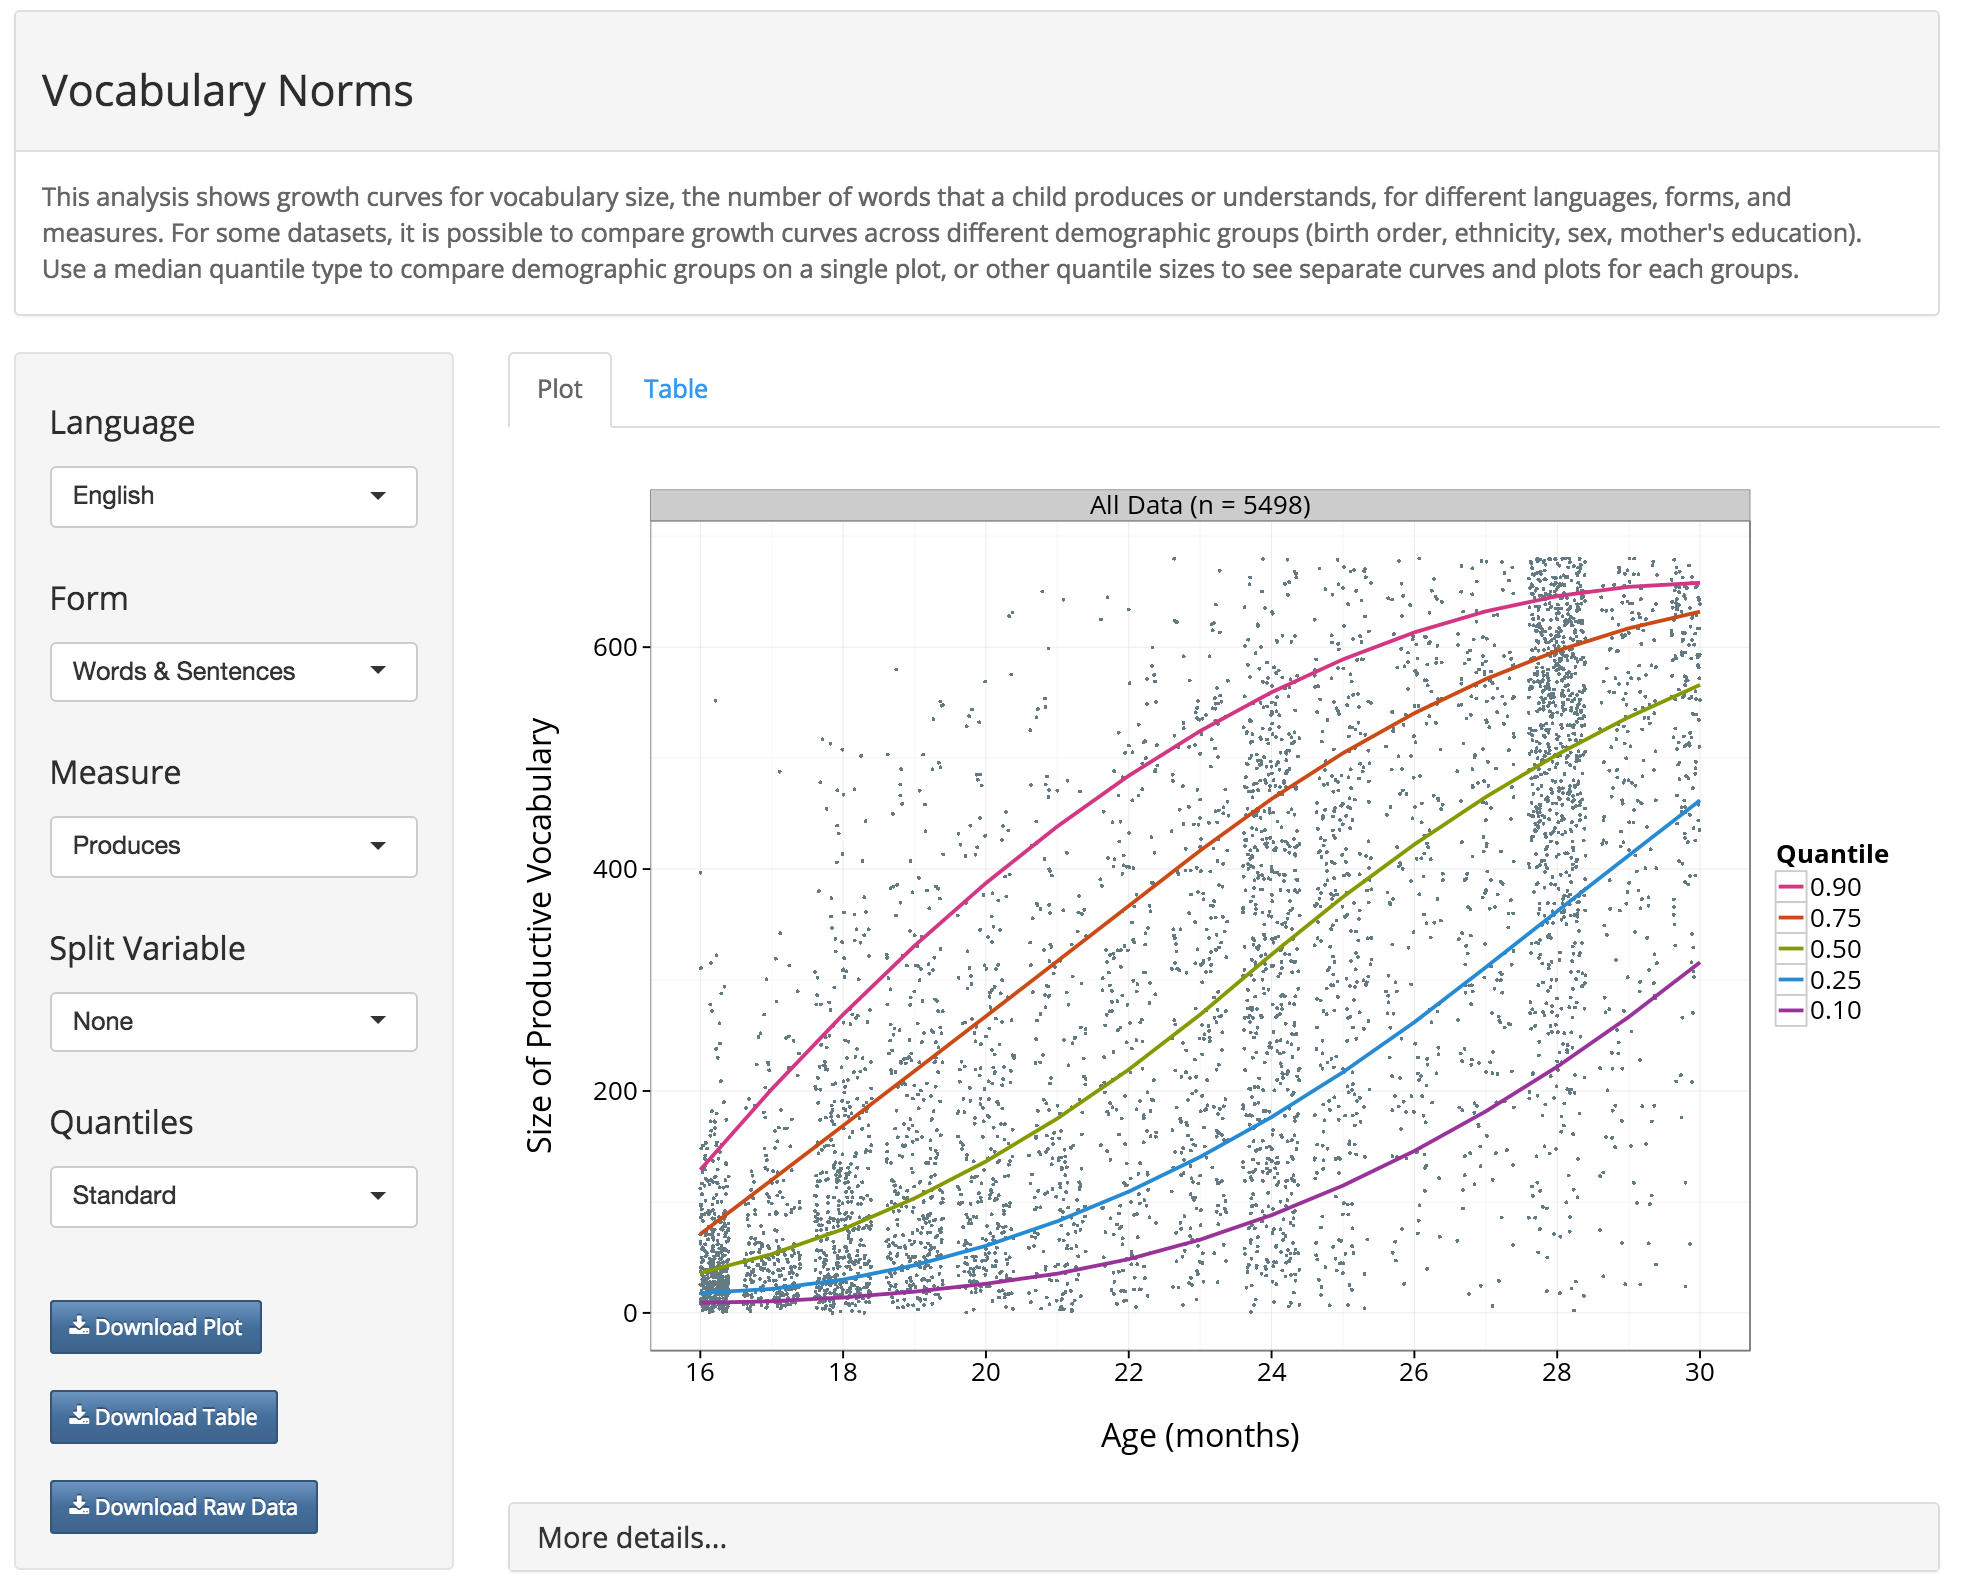
\includegraphics[width=6.5in]{figures/normsapp.png}
\caption{\label{fig:norms}.}
\end{figure}


\subsubsection{Item Trajectories}

\begin{figure}[h!]
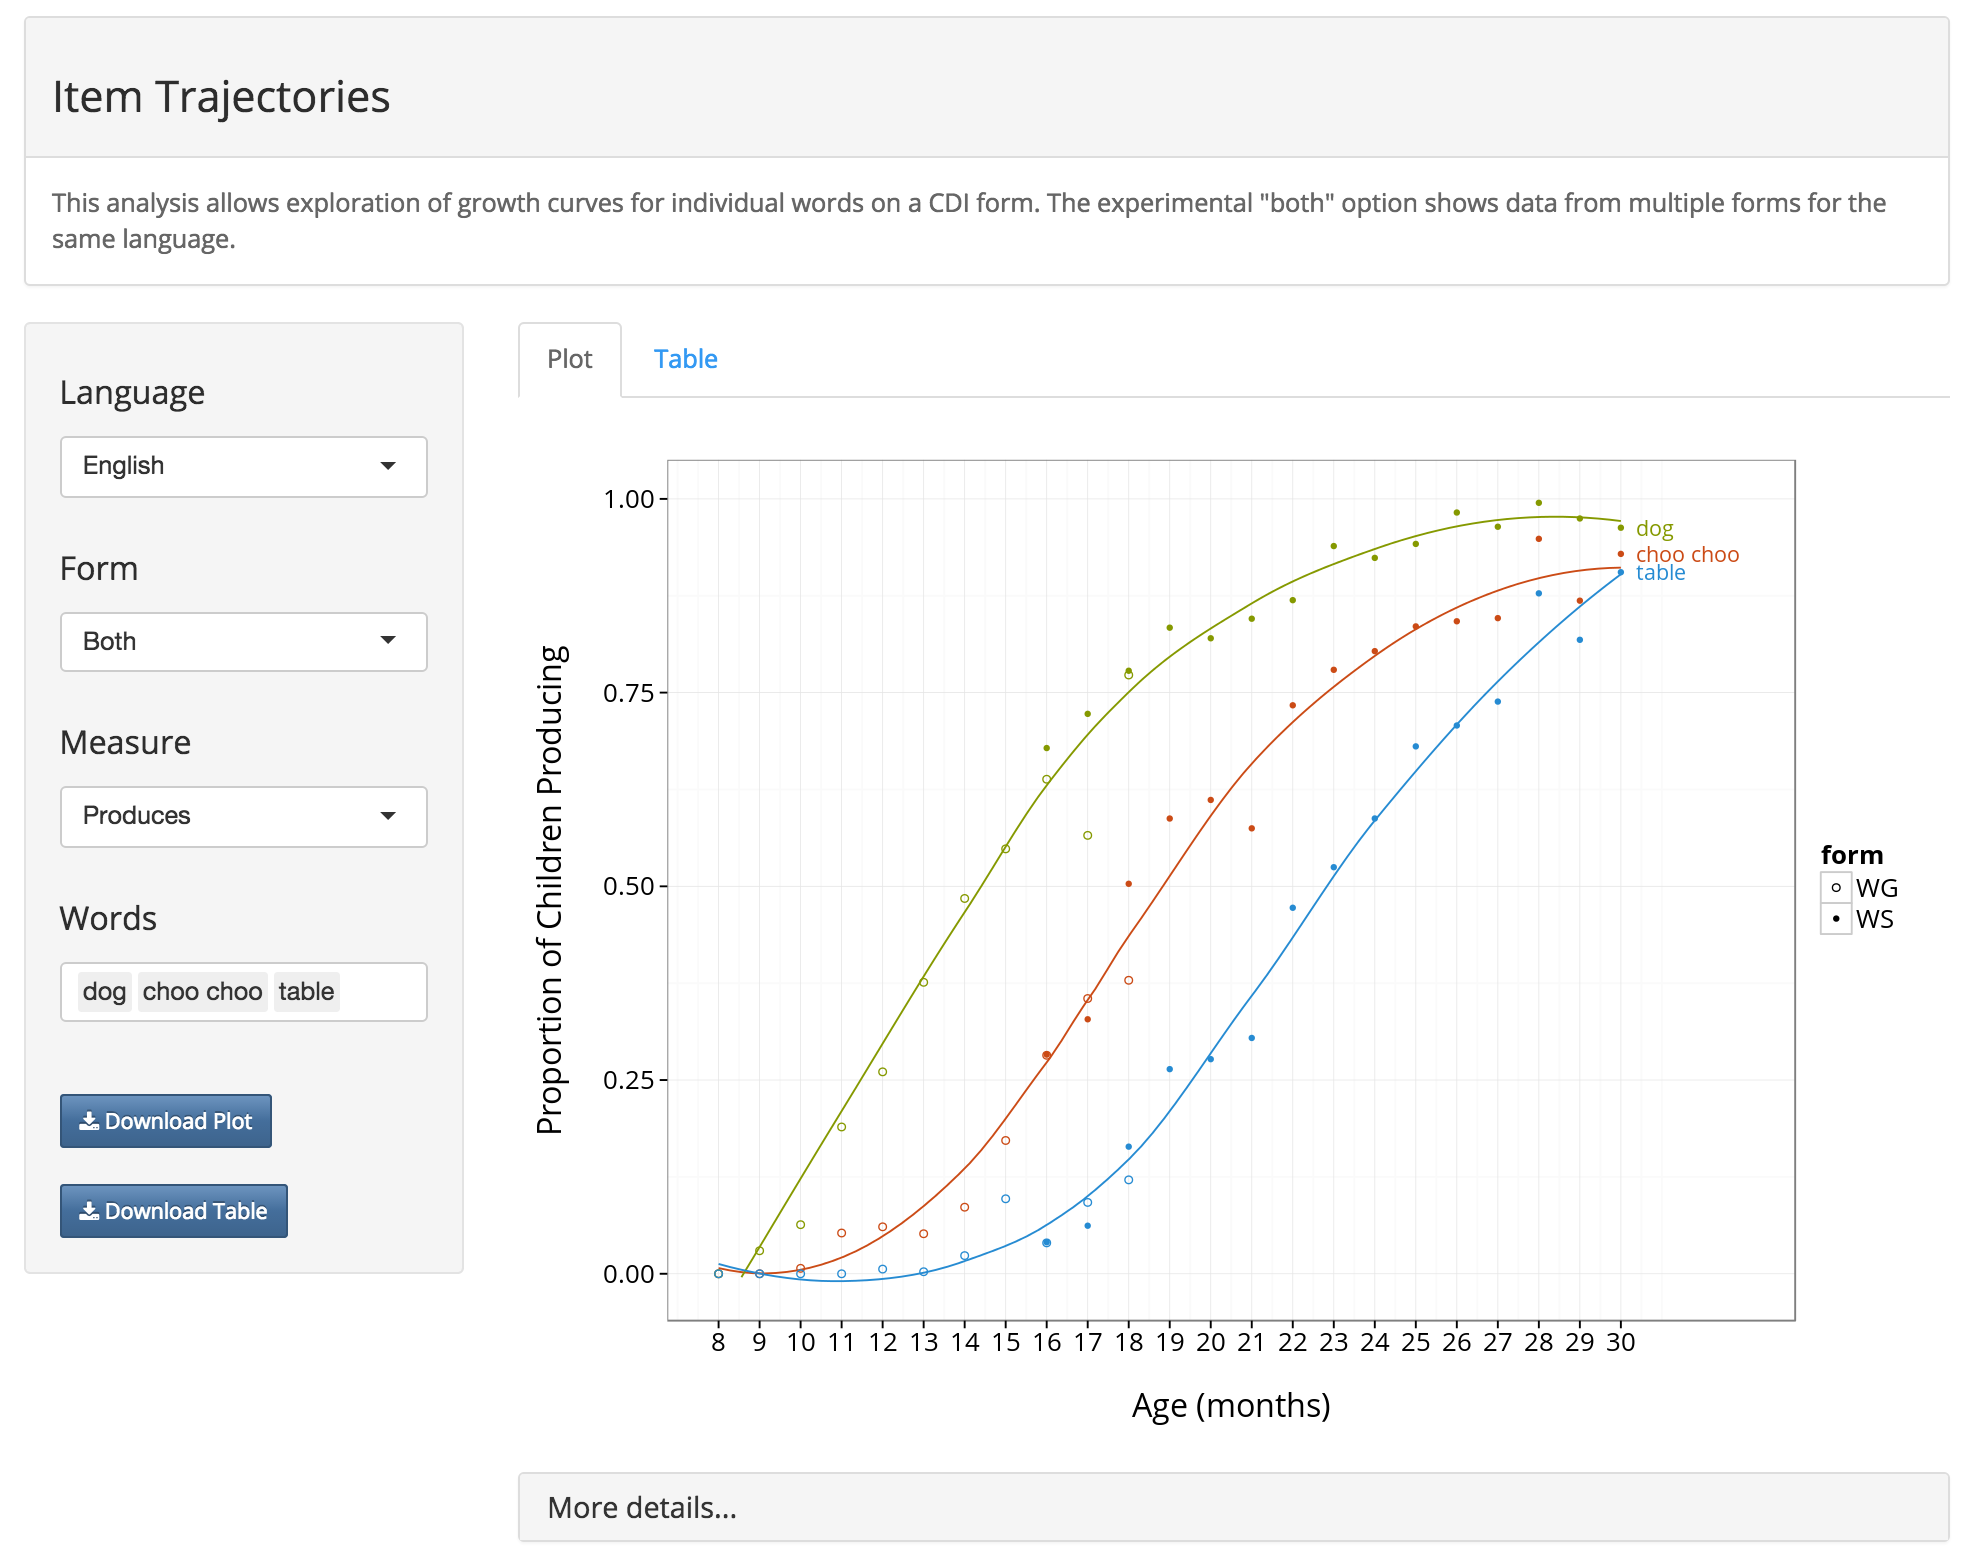
\includegraphics[width=6.5in]{figures/itemsapp.png}
\caption{\label{fig:items} }
\end{figure}


\subsection{Extensibility}


\section{wordbankR: an R package for accessing Wordbank}




\section{Conclusions}

\subsection{Addressing the limitations of parent report}


Although the standardized parent report format contributes to the availability of large amounts of data in a comparable format, there are limitations to the parent report methodology as well \cite{tomasello1994,feldman2000}. We believe that Wordbank has the potential to help address some of these issues.

First, parents may be biased observers, either underestimating or overestimating children's abilities. The CDI instruments were designed to minimize bias, targeting current and emerging behaviors and asking parents about highly salient features of their child's abilities. As such, they yield reliable and valid estimates of developing language skills, with dozens of studies demonstrating concurrent and predictive relations to naturalistic and observational measures in both typically-developing and at-risk populations \cite<e.g.,>{dale1996, thal2000, marchman2002}. Yet, there is also evidence that some variability may be due to reporting biases linked to factors such as SES \cite{feldman2000,fenson2000,feldman2005}. Increasing overall sample sizes from diverse populations can both improve the precision of estimates across the full population and allow analyses to disentangle measurement artifacts from systematic bias related to sub-population characteristics. 
		
Second, the items on the original CDI instruments were chosen to be a representative sample of vocabulary for the appropriate age and language \cite{fenson1994}, not with the intention that they would be a universal set of words that could be compared across instruments. Accordingly, while statistical corrections for word-list size do exist \cite{mayor2011}, our approach in Wordbank is conservative with respect to comparisons across instruments and languages. All analyses reported below are \emph{within-form} analyses---only standardized and aggregated patterns (e.g. correlations between items, quantile comparisons) are compared across forms. Such comparisons do not require problematic assumptions about translation equivalence (see Sec. \ref{sec:architecture}).

Third, the original norming study for the English CDIs was published in 1994, based on a sample of more than 1800 children. While a heroic effort, this sample was limited in its geographic and demographic representation, most notably including a high proportion of families who were college-educated. The Advisory Board later expanded these norms to be more broadly representative of the US population, adding more than 800 children \cite{fenson2007}. Nevertheless, this new sample still includes substantial underrepresentation of children whose mother did not complete high school (15\% in census norms, 7\% in updated CDI norms) and overrepresentation of White families (64\% in census norms, 73\% in updated CDI norms). By expanding the SES representation, as well as including a range of populations, Wordbank aims to improve the utility of the CDI.

Finally, while the CDI inventories were not designed to provide individually-reliable estimates of children's knowledge of particular words, we nevertheless believe that with enough data, we can extract meaningful information about word knowledge. In particular, analyses of item-level correlations using CDI data has provided insightful leverage on outcome measures with far smaller samples than we have available \cite{hills2009,hills2009b,hills2010,beckage2011}; thus, we believe that Wordbank-scale data will provide precision at the item level as well as at the level of the whole vocabulary.


\bibliographystyle{apacite}
\bibliography{wordbank}

\end{document}
